\section{Bilder} \label{sec:bilder}
Bilder i programmet følger med boligobjektet, bildene blir ikke lagret i selve objektet og serialiseres ikke. Referanse til bildemappen er samme som static variabeln \emph{objektID}. Første bilde som brukeren laster opp blir brukt på fremsiden ved presentasjon av boligen. Dette bilde blir plassert i boligmappen som 1.jpg, dersom brukeren velger å laste opp flere bilder får de inkrementelle navn som 2.jpg, 3.jpg og så videre. 

\subsection{Bildeklasser}
\subsubsection*{Bildefilsti.java}
Primær oppgave for klassen er å sørge for at programmer får en absolutt filsti til hvor alle bilder er lagret. Metoder i denne klasse returnerer en \emph{String} som i sin tur benyttes i \emph{File()} objekter tværs over programmet.  
Klassen ble oprettet på grunn av at html visninger stiler krav på en absolut filsti for html som i tilleg begynner med "<file:">. Derfor metoder i klassen kan: 
\begin{itemize}[noitemsep,nolistsep]
\item Returnere plassering til \texttt{programdata/img/} uavhengig operativsystem.
\item Returnere filsti til et standard bilde som vises dersom brukeren ikke laster opp egne bilder.
\item Gitt et boligobjekt:
\begin{itemize}
\item Filsti til boligens fremsidebilde som kan brukes i File() og som html sti\footnote{Som beskrevet over blir strengen returnert med prefix "<file:">}
\item Filsti til boligens gallerimappe og som html sti
\end{itemize}
\end{itemize}

\subsubsection*{BoligBilde.java}
Klassen brukes til bildebahendlig og opplastning av bilder til eksisterende boligobjekter. Metoder i klassen (1) kontrollerer antall alerede opplastede bilder for boligen, (2) leser inn nytt bilde fra harddisk (gitt et \emph{File()} objekt), (3) endrer størrelsen på bildet slik at det blir tilpasset den visning som brukes i programmet (også for å holde størrelsen nede på bildemappen), (4) lagrer behandlet bile i gallerimappen for boligen.

\subsection{Lagring av bilder}
Lagring av bilder er ikke serialisert hvilket medfører at alle bilder blir lagret som bildefiler i \texttt{programdata/img/\textbf{objektID}}. For hver boligobjekt som blir oprettet lages det en ny mappe med samme navn som \emph{objektID}. Dette gjør at men unngår serialisering av bildeobjekter samt start og avslutting av programmet blir betydelig raskere. Etter at bildemappe er opprettet kan brukeren legge til bilder for boligen. Logikken foretar følgende trinn ved opplastning av bilde for en bolig:
\begin{enumerate}[noitemsep,nolistsep]

\item Fra vindu for boligregistrering/endring brukeren initierer \emph{JFileChooser} dersom man velger å laste opp bilder. her blir det gjort forskjell på dersom dette er en ny bolig eller et eksisterende bolig slik at brukeren får se riktig dialog etter at registrering av en ny bolig er klar.

\item Dersom brukeren laster opp en ny fil blir dette buffret som \emph{BufferedImage} og endret størrelse på, eksepel \ref{kode:innlesningbilde} og \ref{kode:bildestorrelse}.

\item Etter endring av størrelse blir bildet lagret med inkrementelt filnummer fra forrige bilde. Dersom det ikke finnes bilder med fra tidligere blir det satt til 1.jpg, eksempel \ref{kode:bildelagring}.

\end{enumerate}

\begin{lstlisting}[caption=BoligBilde.java: Innlesning av bildefil, label=kode:innlesningbilde]
	private void lesInnBilde(File bildeFil) throws IOException {
        bilde = ImageIO.read(bildeFil);
        bildeType = bilde.getType() == 0 ? BufferedImage.TYPE_INT_ARGB : bilde.getType();
    }
\end{lstlisting}

\begin{lstlisting}[caption=BoligBilde.java: Endring av opplastet bildestørrelse, label=kode:bildestorrelse]
	private BufferedImage endreBildeTilStandardStorrelse(BufferedImage originalBilde, int bildeType) {
        BufferedImage nyttBilde = new BufferedImage(Konstanter.BILDE_WIDTH, Konstanter.BILDE_HEIGHT, bildeType);
        Graphics2D grafikk = nyttBilde.createGraphics();
        grafikk.drawImage(originalBilde, 0, 0, Konstanter.BILDE_WIDTH, Konstanter.BILDE_HEIGHT, null);
        grafikk.dispose();
        return nyttBilde;
    }
\end{lstlisting}

\begin{lstlisting}[caption=BoligBilde.java: Lagring av et nytt eller tillegsbilde for en bolig, label=kode:bildelagring]
	private void lagreBilde(BufferedImage bilde, String path) throws IOException {
        ImageIO.write(bilde, "jpg", new File(path));
    }

	public void lagreNyttBildeForBolig(Bolig bolig, File innlestFil) throws IOException {
        lesInnBilde(innlestFil);
        BufferedImage tmpBilde = endreBildeTilStandardStorrelse(bilde, bildeType);
        String galleriSti = getGalleriSti(bolig);
        String fullSti = galleriSti + "/" + String.valueOf(getNesteFilnummer(bolig)) + ".jpg";
        lagreBilde(tmpBilde, fullSti);
    }
\end{lstlisting}

\subsection{Visning av bilder}
Bildevisning kan initialiseres på tre forskjellige måter, fra vindu for boligbehandling, figur \ref{fig:bildebahndling} der megleren får mulighet til å laste opp nye boliger eller starte en bildevisning for alrede registrerte bolider for den eksisterende boligen. Dersom brukeren laster opp et bilde blir man også presentert med en dialog med spørsmål om å registrere flere bilder på samme bolig, se figur \ref{fig:lasteoppbilder}. Den andre og siste metoden for å starte en bildevisning er å klikke i visningsvindu til megler eller boligsøker. Dette vil da hente opp visningsvindu for bildene som er presentert i figur \ref{fig:bildevisning}.
Dersom brukeren velger å ikke laste opp minst et bilde for en bolig blir kommer metoden \emph{BoligBilde.antallBilder} til å raportere 0 og derigjennom blir det hentet et standardbilde fra \texttt{./programdata/img/default/1.jpg} og presentert både i annonser og i bildevisningen. Se figur \ref{fig:manglerbilde}. 


\begin{figure}[ht!]
\center
 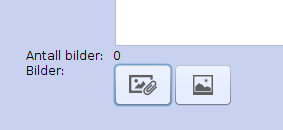
\includegraphics{./img/produktdokumentasjon/bilder/1.png}
 \caption{Utsnitt fra boligbehandlingsvindu. Viser kontroller for opplastning og visning av bilder som er registrert for dette bildeobjektet.}
 \label{fig:bildebahndling}
\end{figure}

\begin{figure}[ht!]
 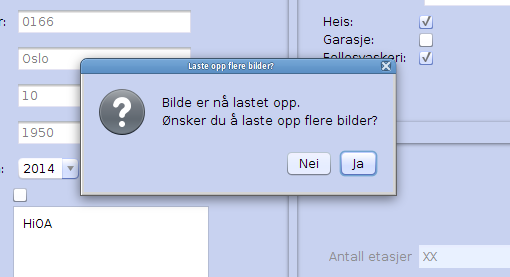
\includegraphics[width=\textwidth,height=\textheight,keepaspectratio]{./img/produktdokumentasjon/bilder/2.png}
 \caption{Utsnitt fra boligbehandlingsvindu. Viser forespørsel til bruker (megler) dersom den ønsker å laste opp flere bilder for boligobjetet.}
 \label{fig:lasteoppbilder}
\end{figure}

\begin{figure}[ht!]
 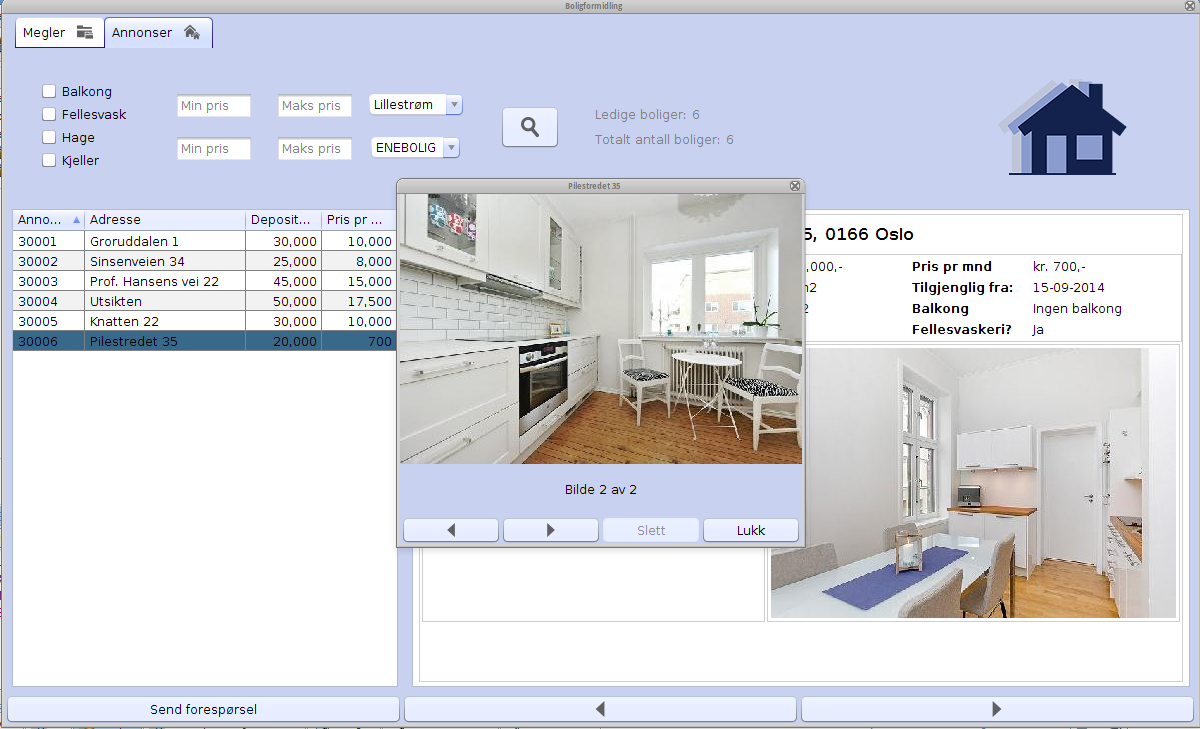
\includegraphics[width=\textwidth,height=\textheight,keepaspectratio]{./img/produktdokumentasjon/bilder/3.png}
 \caption{Bildevisning initialisert gjennom klikk i visningsarea for boligsøker.}
 \label{fig:bildevisning}
\end{figure}

\begin{figure}[ht!]
 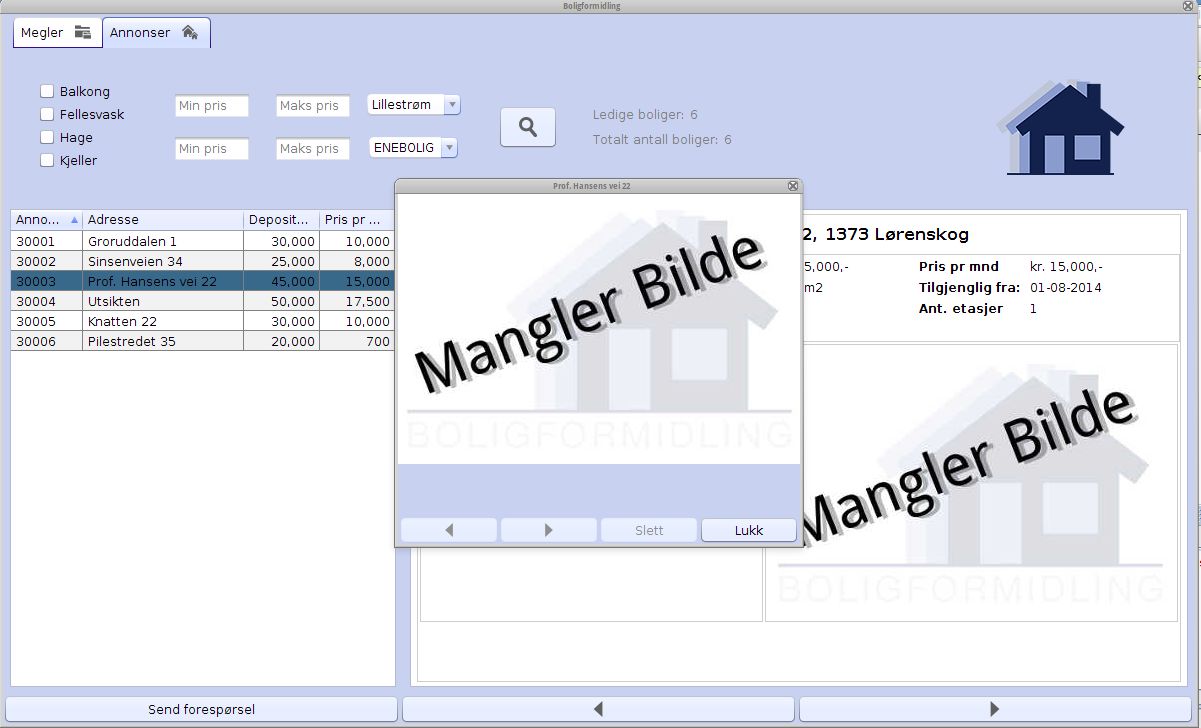
\includegraphics[width=\textwidth,height=\textheight,keepaspectratio]{./img/produktdokumentasjon/bilder/4.png}
 \caption{Eksepel på standardbilde som vises dersom brukeren ikke har lastet opp et bilde etter registrering av en ny bolig.}
 \label{fig:manglerbilde}
\end{figure}

\subsection{Sletting av bilder}
Sletting av bilder er foreløpig ikke implementert. Dersom et boligobjekt blir slettet må gallerimappen til boligen slettes manuellt. Det er tatt høyde for å implementere sletting og mulighet for dette er satt opp i brukergrensesnitet men foreløpig er deaktivert. 